% =====================================================================
%  Artigo do seminário -- modelo IEEE conference (duas colunas)
%  Estrutura:
%    Main.tex              -> arquivo principal (compile este)
%    config/pacotes.tex    -> pacotes e configurações de formatação
%    config/comandos.tex   -> macros e símbolos próprios do artigo
%    Capitulos/*.tex       -> uma seção por arquivo
%    images/               -> figuras
%    artigo.bib            -> referências (biblatex + biber)
% =====================================================================
\documentclass[conference]{IEEEtran}

% =====================================================================
%  Pacotes e configurações de formatação
% =====================================================================

% ---------- Idioma e codificação ----------
\usepackage[utf8]{inputenc}
\usepackage[T1]{fontenc}
\usepackage[portuguese]{babel}

% ---------- Fontes (Times, como no padrão IEEE) ----------
\usepackage{newtxtext}
\usepackage{newtxmath}
\usepackage{microtype}

% ---------- Matemática e unidades ----------
\usepackage{amsmath}
\usepackage{bm}
\usepackage[
    output-decimal-marker={,},
    group-separator={.},
    per-mode=symbol,
    range-phrase={ a },
    list-final-separator={ e },
    list-pair-separator={ e }
]{siunitx}

% ---------- Figuras, tabelas e diagramas ----------
\usepackage{graphicx}
\usepackage{xcolor}
\usepackage{booktabs}
\usepackage{array}
\usepackage{multirow}
\usepackage{tikz}
\usetikzlibrary{arrows.meta,positioning,calc}

\graphicspath{{./images/}}

% ---------- Listas ----------
\usepackage{enumitem}
\setlist[itemize]{label=\textbullet, leftmargin=*, itemsep=2pt, topsep=4pt}
\setlist[enumerate]{label=\arabic*., leftmargin=*, itemsep=2pt, topsep=4pt}

% ---------- Links e referências cruzadas ----------
\usepackage{url}
\usepackage[autostyle=false,style=english]{csquotes} % aspas “ ” nas referências
\usepackage[hidelinks]{hyperref}

% ---------- Bibliografia (estilo IEEE: [1], [2], ...) ----------
\usepackage[style=ieee,backend=biber,sorting=none,maxnames=6]{biblatex}
\addbibresource{artigo.bib}
\renewcommand*{\bibfont}{\footnotesize}

% ---------- Rótulos em português no padrão IEEE ----------
% Figuras ficam como "Fig. 1." e tabelas como "TABELA I" (padrão do IEEEtran).
\renewcommand{\IEEEkeywordsname}{Palavras-chave}
\addto\captionsportuguese{%
    \renewcommand{\abstractname}{Resumo}%
    \renewcommand{\tablename}{TABELA}%
    \renewcommand{\figurename}{Fig.}%
}




\usepackage{indentfirst}   % recuo também no 1º parágrafo após \section
% =====================================================================
%  Macros do artigo
%  Defina aqui símbolos usados várias vezes para manter a notação única.
% =====================================================================

% Fasores e vetores em negrito: \fasor{V}
\newcommand{\fasor}[1]{\mathbf{#1}}

% Subscritos em texto (não itálicos): V_{\sub{dc}}
\newcommand{\sub}[1]{\mathrm{#1}}

% Abreviações recorrentes
\newcommand{\FP}{\mathrm{FP}}
\newcommand{\THD}{\mathrm{THD}}

% Título em itálico no início de parágrafo (como em "Limitações." no modelo)
\newcommand{\paragrafo}[1]{\textit{#1.}\ }


% ---------- Título e autores ----------
\title{Modelo de Controle de um Retificador de Vienna Trifásico a Quatro Fios com Fator de Potência Variável}

\author{%
    \IEEEauthorblockN{Vitor Gabriel Saturnino de Melo}
    \IEEEauthorblockA{Escola de Engenharia de São Carlos\\
    Universidade de São Paulo (EESC-USP)\\
    São Carlos, SP, Brasil}
    \and
    \IEEEauthorblockN{João Pedro Muto Cisotto}
    \IEEEauthorblockA{Escola de Engenharia de São Carlos\\
    Universidade de São Paulo (EESC-USP)\\
    São Carlos, SP, Brasil}
}

\begin{document}

\maketitle

% ---------- Resumo e palavras-chave ----------
\begin{abstract}
O retificador de Vienna é uma das topologias mais utilizadas em estágios de 
conversão CA-CC, em especial em carregadores de veículos elétricos (VEs) de média
e alta potência. Nesse sentido, este trabalho revisa topologias de conversores com correção
de fator de potência (PFC) aplicadas a VEs e detalha a topologia do retificador de
Vienna trifásico a quatro fios (ponto de neutro aterrado) com fator de potência variável.
Tendo isso em mente, é apresentado um modelo por fase e uma estrutura de controle para o 
retificador citado anteriormente, na qual são desenvolvidos controladores proporcional-ressonantes (PR)
de corrente para cada fase, um controlador proporcional-integral (PI) para o controle da tensão do barramento CC e
um controlador PI para o controle do equilíbrio do ponto médio e geração de referência com 
fator de potência (FP) variável. Por fim, são apresentadas simulações de um conversor de \SI{21}{kW},
que demonstram a eficácia do modelo e da estratégia de controle propostos, obtendo um THD inferior a \SI{2}{\percent} após o controle.
\end{abstract}

\begin{IEEEkeywords}
retificador de Vienna, fator de potência variável, controle ressonante, carregadores de veículos elétricos.
\end{IEEEkeywords}

% ---------- Seções ----------
\section{Introdução}
\label{sec:introducao}

Em carregadores de veículos elétricos o estágio de entrada precisa absorver uma corrente
senoidal com FP elevado e baixo THD, dentro das normas estabelecidas pela IEEE 519 \cite{ieee519}
e fornecer um barramento CC regulado ao conversor CC-CC que alimenta a bateria. Os conversores PFC monofásicos, 
como o \textit{boost}, o \textit{bridgeless} e o \textit{totem-pole}, são amplamente utilizados em carregadores de baixa potência,
porém em estações de recarga rápidas ou carregadores embarcados que operam na faixa de \SI{20}{kW}, faz-se necessária a utilização
de retificadores trifásicos multiníveis, como o retificador de Vienna, para reduzir os esforços nas chaves semicondutoras e o tamanho de filtros utilizados \cite{yilmaz2013review,tu2019extreme}.

O retificador de Vienna se destaca nesse cenário por utilizar apenas três chaves bidirecionais, que bloqueiam metade da tensão do barramento, 
dessa forma diminuindo o estresse nas chaves e permitindo a utilização de semicondutores de menor tensão nominal \cite{safayatullah2022comprehensive}, sendo amplamente utilizado em módulos comerciais de recarga rápida.

O retificador de Vienna a quatro fios (ponto de neutro aterrado) com fator de potência variável é uma topologia em que o neutro da rede é ligado ao ponto médio do barramento \cite{alahuhtala2006fourwire}, essa conexão permite
que o conversor opere com cargas e redes desequilibradas, tendo em vista que ele fixa o potencial do ponto médio (o que reduz o ruído de modo comum) e viabiliza sua utilização em redes monofásicas e trifásicas \cite{schafmeister2021transformerless}. 
Além disso, retificadores unidirecionais, além de poderem operar com PFC, podem oferecer serviços à rede como compensação de reativo e FP ajustável. 
Nesse sentido, este trabalho visa o desenvolvimento de uma estrutura de controle de um retificador de Vienna trifásico a quatro fios no referencial estacionário, com PR por fase e FP variável desacoplado da malha de tensão.

\section{Revisão Bibliográfica}
\label{sec:revisao}

\subsection{Arquiteturas de recarga de veículos elétricos}
Os carregadores de veículos elétricos podem ser classificados em embarcados (\textit{on-board},OBC) que operam tipicamente entre 3,7 kW e 22 kW e a externos (\textit{off-board})
de dezenas a centenas de kW \cite{yilmaz2013review,tu2019extreme}. Ambos tipos 
apresentam dois estágios, o primeiro é um retificador PFC que é responsável por regular 
o barramento CC intermediário e o seguindo é um conversor CC-CC isolado que adapta a tensão do barramento CC à tensão da bateria (tipicamente entre 400 e 800 V). 

Estações de recarga rápidas apresentam o estágio CA-CC formado por módulos de 15 a 30 kW em paralelo para diminuir o esforço das chaves dos retificadores, sendo a escolha da 
topologia utilizada dependente da eficiência, densidade de potência e qualidade de energia necessária. Como os 
OBCs podem operar tanto em redes monofásicas quanto em redes trifásicas, topologias com
o ponto médio do barramento ligado aso neutro da rede são comumente utilizadas \cite{schafmeister2021transformerless}.
\subsection{Topologias de retificadores trifásiocos}

Existem diversas topologias de retificadores trifásicos, entre elas podem ser destacadas algumas características. 

As pontes de diodos com conversor boost são simples e necessitam de apenas uma chave, por conta dessa particularidade, apresentam
apenas um nível de tensão e um fluxo de corrente unidirecional, não sendo possível controlar o FP, o que provoca
uma corrente de linha distorcida. As topologias de retificador com PWM de dois níveis apresentam seis chaves e são bidirecionais, além de apresentarem
dois níveis de tensão, permitindo o controle completo do fator de potência e da corrente de linha, porém apresentam uma maior complexidade de controle e suas chaves bloqueiam a tensão do barramento, assim ficam sobre um estresse maior \cite{kolar2013essence}. 

Já as topologias NPC/tipo-T apresentam doze chaves e 3 níveis de tensão, além de permitirem um fluxo de corrente
bidirecional, o que torna possível a operação em modo de recarga e de injeção de energia na rede. Apesar de reduzirem os esforçoes sobre cada chave, seu custo é maior
tendo em vista a necessidade de doze chaves \cite{safayatullah2022comprehensive}. O retificador de Vienna de três fios \cite{kolar1997novel} é a versão unidirecional do 
tipo-T, ele apresenta três chaves bidirecionais e seis diodos rápidos que produzem três níveis de tensão, com bloqueio de tensão em $V_{\sub{dc}}/2$. Esse comportamento garante uma alta eficiência e alta densidade de potência, porém não permite a operação bidirecional 
e o controle de fator de potência é limitado. O retificador de Vienna de 4 fios foi proposto, especialmente no contexto de carregamento de veículos elétricos, tendo em vista sua aplicação em estações de recarga rápidas fora do veículo \cite{senthilkumar2025iipq} e
para carregadores embarcados sem transformados \cite{schafmeister2021transformerless}. Assim como o retificador de Vienna de três fios, o retificador de Vienna de quatro fios apresenta três níveis de tensão, porém com a adição de um quarto fio, o neutro da rede, é possível controlar o fator de potência da rede, seu fluxo de corrente é unidirecional e apresenta 3 níveis de tensão.

\subsection{Estratégias de controle}

Para um retificador de Vienna de quatro fios, os mecanismos doe controle, de forma geral, se concentram em três malhas, uma para a corrente de entrada,
uma para a tensão do barramento CC e uma para o equilíbrio do ponto médio do barramento CC. A malha de corrente de entrada é responsável por controlar a corrente de linha, garantindo que ela siga uma referência senoidal em fase com a tensão da rede, o que permite o controle do fator de potência. A malha de tensão do barramento CC regula a tensão do barramento intermediário, garantindo que ela permaneça dentro dos limites especificados para a operação segura do conversor. Por fim, a malha de equilíbrio do ponto médio do barramento CC assegura que as tensões nos capacitores do barramento permaneçam equilibradas, evitando sobrecargas em um dos capacitores e garantindo a estabilidade do sistema.

Para o retificador destacado anteriormente, o equilíbrio é realizado com um termo aditivo na amplitude da referência, com sinal dependente do semiciclo \cite{alahuhtala2006fourwire}.


\section{Topologia e Modelo Matemático}
\label{sec:modelo}

\begin{figure}[!t]
    \centering
    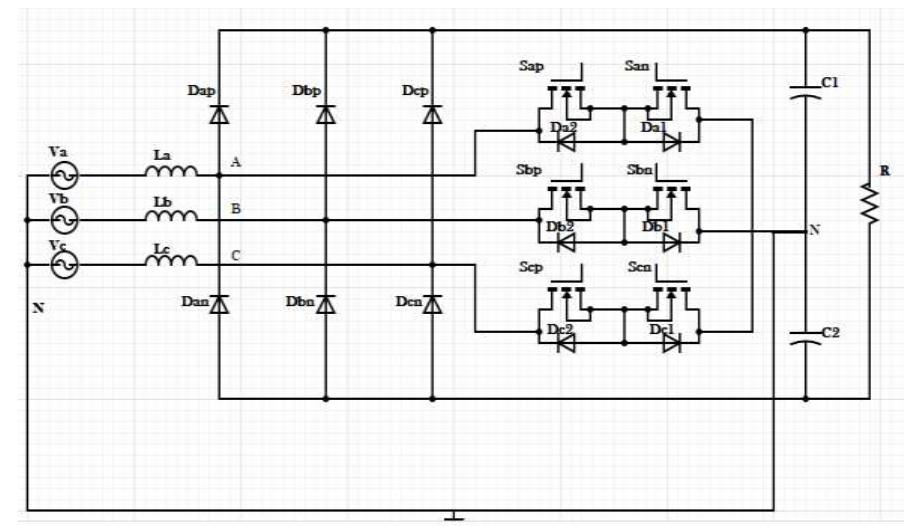
\includegraphics[width=\linewidth]{images/figure-3-phase-wire-vienna-rectifier.jpeg}
    \caption{Braço do Vienna de 4 fios.}
    \label{fig:braco_vienna}
\end{figure}

A figura \ref{fig:braco_vienna} mostra o braço do retificador de Vienna de quatro fios,
a tensão aplicada à fase é a tensão de polo $v_{kM}$, e cada fase  $k \in \{a,b,c\}$ é descrita de forma independente, como apresentado na equação \ref{eq:modelo_vienna4}.

\begin{equation}
    L\frac{di_k}{dt} = v_k - R i_k - v_{kM}, \qquad
    v_{kM} =
    \begin{cases}
        (1-d_k)V_{C1},  & i_k > 0\\
        -(1-d_k)V_{C2}, & i_k < 0
    \end{cases}
    \label{eq:modelo_vienna4}
\end{equation}

Na equação, $d_k$  é a razão cíclica da chave $S_k$. Além disso, os capacitores respeitam a
equação \ref{eq:capacitores}.

\begin{equation}
    C\frac{dV_{C1}}{dt} = \sum_{i_k>0}^{}(1-d_k)i_k-i_L, \qquad
    C\frac{dV_{C2}}{dt} = \sum_{i_k<0}^{}(1-d_k)|i_k|-i_L.
    \label{eq:capacitores}
\end{equation}

Da equação \ref{eq:modelo_vienna}, tem-se que a corrente no ponto médio ($i_M$) é a soma das correntes de cada fase, ou seja, $i_M = \sum_{}^{}d_ki_k$. 
Além disso, em regime permantente, o conversor deve sintetizar uma tensão, que no formato de fasores, pode ser representada por:

\begin{equation}
    \fasor{V}_{\sub{conv}} = \fasor{V}_s - (R + j\omega_0 L)\fasor{I}, \fasor{I} = Ae^{-j\phi},
    \label{eq:fasor}
\end{equation}

Na equação \ref{eq:fasor}, $\phi>0$ representa uma corrente atrasada. Caso $\fasor{V_{conv}}$ e $\fasor{I}$ não estejam em fase,
então para cada semiciclo, existe um intervalo em que a tensão necessária tem o sinal oposto ao da corrente
e, dessa forma, a corrente irá se distorcer em decorrência da saturação de $d_k$. Desconsideranto R na equação \ref{eq:fasor}, o alinhamento
entre a corrente e a tensão do conversor exige que $V_{pk}sin(\phi) = \omega_{0}LA$, ou seja, a corrente de linha é atrasada em relação à tensão do conversor.
Tendo isso em vista, tem-se a equação \ref{eq:phi}.

\begin{equation}
    \phi= \Psi_0 = arcsin(\omega_0LA/V_{pk})
    \label{eq:phi}
\end{equation}

Logo, o ângulo sem distorção é indutivo e cresce com a corrente.



\section{Estratégia de Controle}
\label{sec:controle}

\subsection{Referências com FP variável}
\obs{revisar depois (talvez simplificar/diminuir)}
No controle por fase adotado, cada corrente é controlada por um PR no
referencial estacionário. A referência de cada fase precisa, portanto, ser
uma senoide definida por uma amplitude e um ângulo, e não por componentes
$d$ e $q$. Ela é escrita como
\begin{equation}
    \begin{gathered}
        i_k^* = A\cos(\theta_k-\varphi) + I_{\sub{bias}}\,\lvert\cos(\theta_k-\varphi)\rvert,\\
        A = \frac{I_{\sub{pk}}}{\cos\varphi},
    \end{gathered}
    \label{eq:corrente_fase}
\end{equation}

Em que $\theta_k$ é o ângulo da tensão da fase $k$, obtido do PLL;
$\varphi$ é o ângulo de defasagem desejado entre corrente e tensão
($\varphi>0$ para corrente atrasada, isto é, carga indutiva);
$I_{\sub{pk}}$ é a saída do PI de tensão; e $I_{\sub{bias}}$ é a saída do PI de
equilíbrio do ponto médio.

Para entender o papel de cada termo, a primeira parcela de
\eqref{eq:corrente_fase} pode ser expandida:
\begin{equation}
    A\cos(\theta-\varphi) = \underbrace{I_{\sub{pk}}\cos\theta}_{\text{em fase com } v}
    + \underbrace{I_{\sub{pk}}\tan\varphi\,\sin\theta}_{\text{em quadratura com } v}.
    \label{eq:decomp}
\end{equation}

A parcela em fase com a tensão é a corrente ativa, e a parcela em quadratura
é a corrente reativa. Para as três fases, as potências são
\begin{equation}
    P = \tfrac{3}{2}V_{\sub{pk}}I_{\sub{pk}}, \qquad Q = P\tan\varphi .
    \label{eq:potencias}
\end{equation}

Duas consequências decorrem daí. Primeiro, a divisão por $\cos\varphi$ na
amplitude $A$ faz com que a componente ativa seja sempre igual a $I_{\sub{pk}}$,
qualquer que seja $\varphi$. Assim, a potência ativa depende apenas da saída
do PI de tensão, e alterar o fator de potência não perturba a regulação do
barramento: as malhas de tensão e de reativo ficam desacopladas. Segundo,
\eqref{eq:decomp} é exatamente a decomposição usada no controle em $dq$, com
$I_d=I_{\sub{pk}}$ e $I_q=I_{\sub{pk}}\tan\varphi$. Escolher $\varphi$ equivale, portanto,
à cadeia $\FP^*\rightarrow Q^*\rightarrow I_q^*$ do controle vetorial, sem
exigir transformações de coordenadas.

O ângulo é obtido diretamente do fator de potência desejado, cujo sinal
indica o tipo ($\FP^*>0$ indutivo, $\FP^*<0$ capacitivo):
\begin{equation}
    \varphi^* = \operatorname{sgn}(\FP^*)\,\arccos\lvert \FP^*\rvert .
    \label{eq:phi_ref}
\end{equation}
Antes de ser aplicado, $\varphi^*$ passa por dois limitadores em série:
\begin{enumerate}
    \item \textit{Janela de quatro fios}: $\varphi\in[\psi_0-\Delta,\ \psi_0+\Delta]$,
    com $\psi_0=\arcsin(K_xI_{\sub{pk}})$, $K_x=\omega_0LI_b/V_{\sub{pk}}$ e $\Delta=\ang{8}$.
    Fora dessa faixa a tensão que o conversor precisaria sintetizar teria sinal
    oposto ao da corrente, o que distorce a corrente
    (Seção~\ref{sec:modelo}, equação~\eqref{eq:phi}).
    \item \textit{Limite de corrente}: a amplitude não pode exceder o valor
    máximo, $A=I_{\sub{pk}}/\cos\varphi\le I_{\sub{max}}$, o que resulta em
    $\lvert\varphi\rvert\le\arccos(I_{\sub{pk}}/I_{\sub{max}})$. Como a potência aparente é $S = \tfrac{3}{2}V_{\sub{pk}}A$, esse limite equivale a
    $S \le S_{\sub{max}} = \tfrac{3}{2}V_{\sub{pk}}I_{\sub{max}}$, ou seja,
    \begin{equation}
        Q_{\sub{max}} = \sqrt{S_{\sub{max}}^2 - P^2}.
        \label{eq:qmax}
    \end{equation}
\end{enumerate}

Por fim, o termo $I_{\sub{bias}}\lvert\cos(\theta_k-\varphi)\rvert$ de
\eqref{eq:corrente_fase} vem do PI de equilíbrio~\cite{alahuhtala2006fourwire}. Como
$\lvert\cos\rvert=\operatorname{sgn}(\cos)\cos$, ele aumenta a amplitude de um
semiciclo e reduz a do outro. O semiciclo positivo carrega $C_1$ e o negativo
carrega $C_2$, então essa assimetria transfere carga entre os capacitores e
mantém $V_{C1}=V_{C2}$.

\subsection{Malha de corrente com controladores PR}

O retificador de Vienna a quatro fios desenvolvido, possui suas fases desacopladas e a
planta por fase, em pu, pode ser descrita por
\begin{equation}
    G_i(s) = \frac{K_iV_{\sub{dc}}}{2(Ls+R)},
    \label{eq:planta_corrente}
\end{equation}
com $K_i = 1/I_b$. Considerando um ganho proporcional com frequência de cruzamento a
1/10 da frequência de chaveamento ($f_c=f_{\sub{sw}}/10$), $\lvert K_pG_i(j\omega_c)\rvert=1$. Então $K_p$, pode
ser calculado pela equação~\eqref{eq:Kp_corrente}

\begin{equation}
    K_p=\frac{2}{K_iV_{\sub{dc}}}\sqrt{(\omega_cL)^2+R^2}.
    \label{eq:Kp_corrente}
\end{equation}

O controlador ressonante pode ser representado por $2K_{Ih}s/(s^2+\omega_0^2)$, com $K_{Ih} = 2{,}2K_p/(n_{oh}T_0)$, o
que resulta em um tempo de subida de $n_{oh}=0{,}9$ ciclo \cite{alonso2018distributed}. Ao implementá-lo por Tustin,
ele pode ser dado por
\begin{equation}
    r(k) = a_h\left[e(k)- e(k-2)\right]+b_h\,r(k-1)-r(k-2),
    \label{eq:tustin}
\end{equation}
com
\begin{equation}
    a_h = \frac{4K_{Ih}T_s}{4+\omega_0^2T_s^2}, \qquad
    b_h = \frac{8-2\omega_0^2T_s^2}{4+\omega_0^2T_s^2}.
    \label{eq:tustin_coef}
\end{equation}

\subsection{Malha de tensão total e de equilíbrio}

Do balanço de potência nos capacitores, considerando $C_{\sub{eq}}=C/2$, então a planta considerada pode
ser obtida com a equação abaixo:

\begin{equation}
    \begin{gathered}
        G_v(s) = \frac{K_v}{s+p_v},\\
        K_v = \frac{3V_{\sub{pk}}I_b}{2C_{\sub{eq}}V_{\sub{dc}}V_b}, \qquad p_v = \frac{2}{R_LC_{\sub{eq}}}
    \end{gathered}
    \label{eq:planta_tensao}
\end{equation}

O PI de tensão total cancela o polo na carga nominal ($K_{i,v}/K_{p,v}=p_v$) e $K_{p,v} = \omega_{cv}/K_v$, com $f_{cv} = \SI{10}{Hz}$.

\obs{terminar dps. Falta descrever o PI de equilíbrio ($I_{\sub{bias}}$) e o \textit{feedforward} com $V_{C1}/V_{C2}$. Falta também uma tabela de parâmetros ($V$, $L$, $C$, $f_{\sub{sw}}$, $I_b$, $V_b$, $R_L$, ganhos).}

\section{Resultados de Simulação}
\label{sec:resultados}

O sistema foi implementado no Matlab/Simulink utilizando a \textit{toolbox} Specialized Power
Systems, com passo de simulação $T_s/50$ e controle discreto amostrado na frequência de
chaveamento $f_{\sub{sw}}$. O THD foi calculado sobre três ciclos de $i_a$, até a 50ª harmônica.

\subsection{Partida e regime permanente}
Para permitir a pré-carga dos capacitores, o PWM é habilitado em $t=\SI{0,2}{s}$. Após isso,
o controle é totalmente habilitado, podendo-se observar, por meio da Fig.~\ref{fig:tensoes}, que a tensão de barramento ($V_{\sub{dc}}$) atinge
\SI{600}{V} que era a tensão de referência, com um sobressinal de cerca de \SI{20}{V} e as tensões sobre
os capacitores $V_{C1}$ e $V_{C2}$ ficam equilibradas em \SI{300}{V}, com uma ondulação de \SI{\pm 12}{V}. Por fim,
as correntes são senoidais e com cerca de \SI{85,9}{A} de pico.

\begin{figure}[!t]
    \centering
    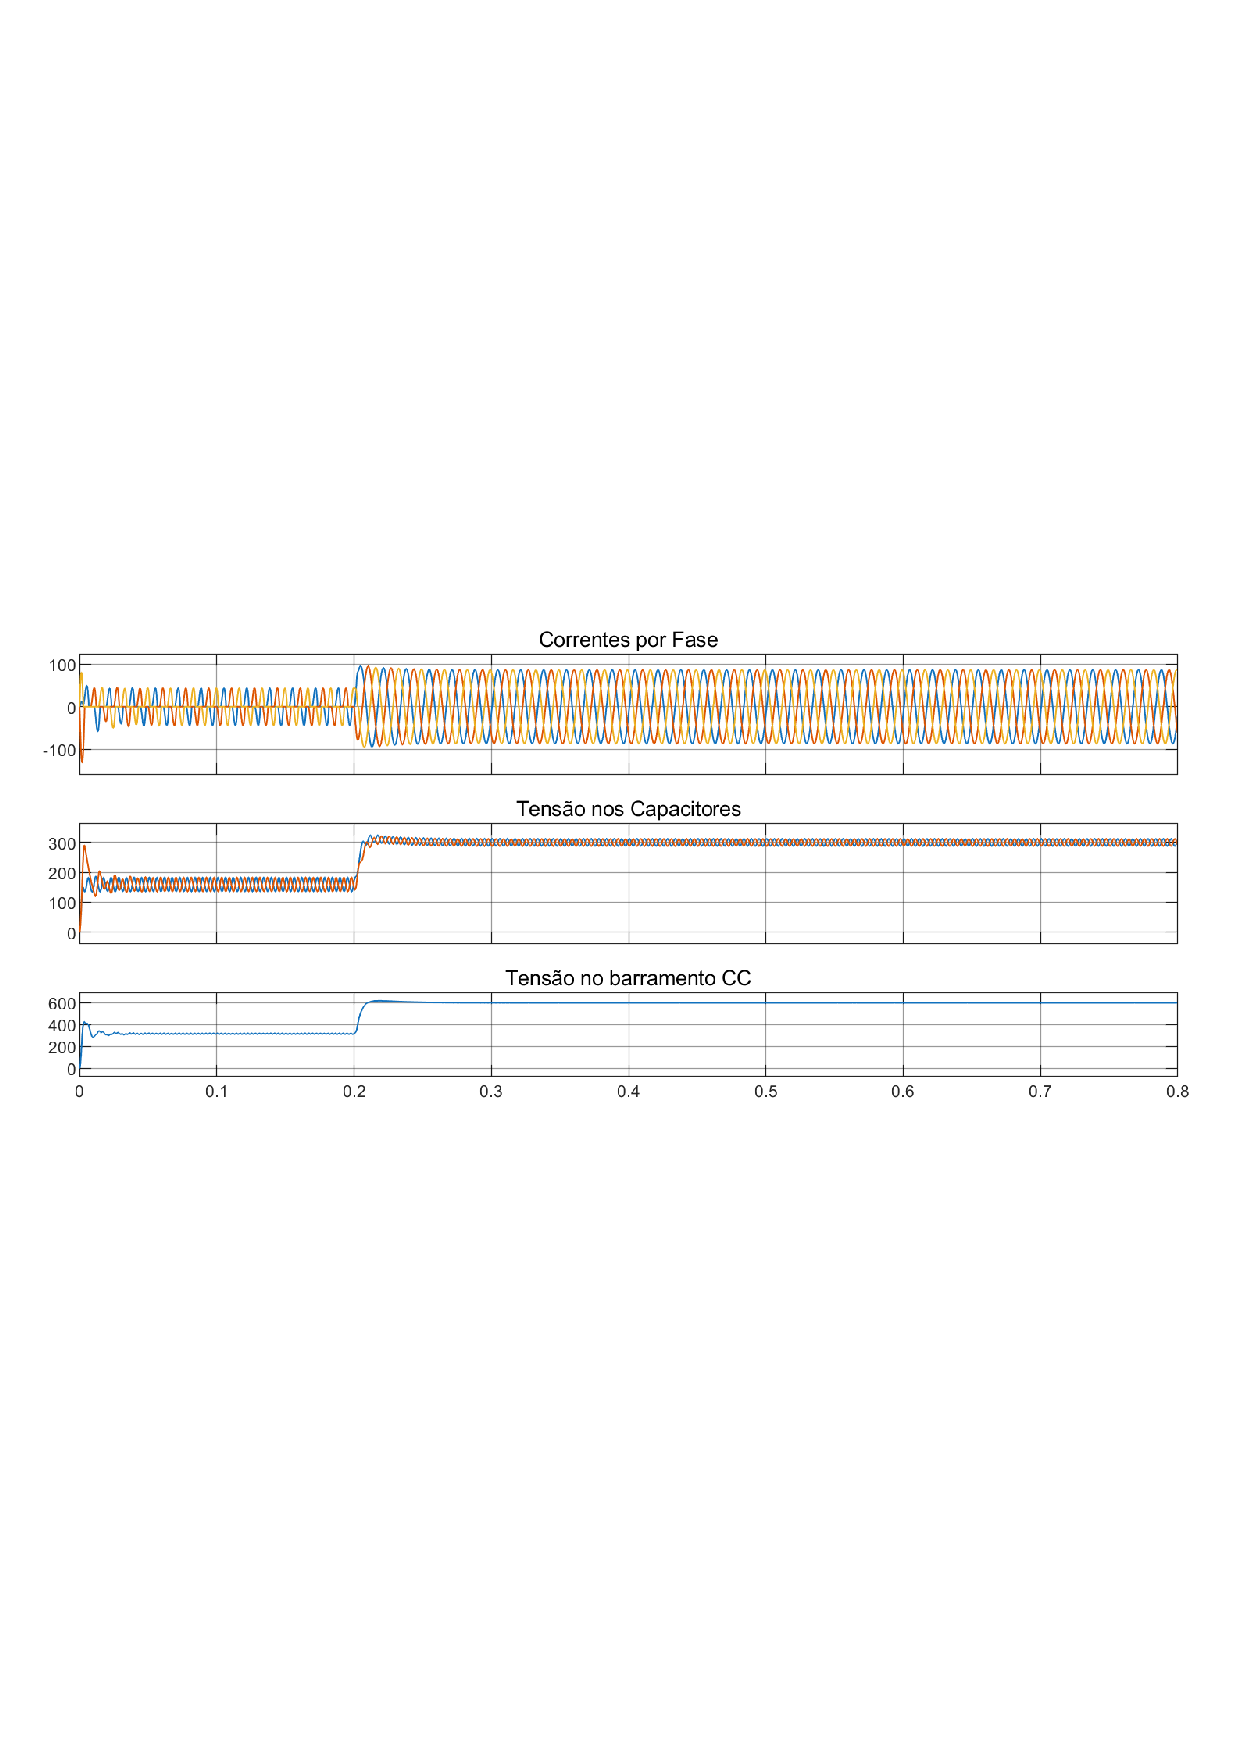
\includegraphics[width=\columnwidth, trim=20 298 20 298, clip]{Tensoes.pdf}
    \caption{Resultados da simulação com limitador ativado.}
    \label{fig:tensoes}
\end{figure}


\subsection{Degraus de Fator de Potência com e sem limitador}

Para verificar se o modelo proposto suportava um PFC, o FP foi variado de 1 para
0,95 indutivo (\SI{0,4}{s}) e depois para 0,95 (\SI{0,6}{s}) capacitivo em carga nominal. Os
resultados são apresentados na Fig.~\ref{fig:potencia} e na Tabela~\ref{tab:res}. Com $\FP^*=1$, o limitador
aplica $\varphi=\ang{7,7}$ e reduz o THD de \SI{7,8}{\percent} para \SI{3,1}{\percent}.

Para o fator de potência em 0,95 indutivo, nota-se que, com e sem limitador, a potência reativa obtida é de \SI{6,8}{kvar} e o FP medido é 0,96, ligeiramente
acima do pedido, pois o reativo é imposto em malha aberta (Tabela~\ref{tab:res}). Nessa situação, é apresentado um THD de \SI{0,3}{\percent}. 

Já para um FP de 0,95 capacitivo, nota-se que, sem limitador, o conversor não é capaz de sintetizar a corrente, uma vez
que conforme discutido na Seção~\ref{sec:modelo}, a tensão necessária teria sinal oposto ao da 
corrente necessária durante cada semiciclo, com isso as razões cíclicas saturam e a corrente se distorce
na passagem por zero
e o THD passa de \SI{20}{\percent}. As harmônicas geradas por essa distorção estão em fase nas três fases e se somam no neutro, elevando
a corrente no neutro e o reativo obtido é menor que o esperado. Com o limitador,
a operação é levada ao limite da janela de operação do retificador ($\varphi \approx \ang{7}$ indutivo), com isso a corrente permanece senoidal, mas o FP medido vai para 0,99 indutivo
conforme é observado nas Figs.~\ref{fig:potencia} e~\ref{fig:potencia2} após \SI{0,6}{s}. A diferença entre o $\FP^*$ e o FP medido é esperada, tendo
em vista que o pedido está fora da região de operação da topologia.

Além disso, pode-se notar também que, em todos os degraus, a potência ativa e a tensão do
barramento CC praticamente não se alteram, o que confirma o desacoplamento previsto anteriormente
em \eqref{eq:decomp}.

\begin{figure}[!t]
    \centering
    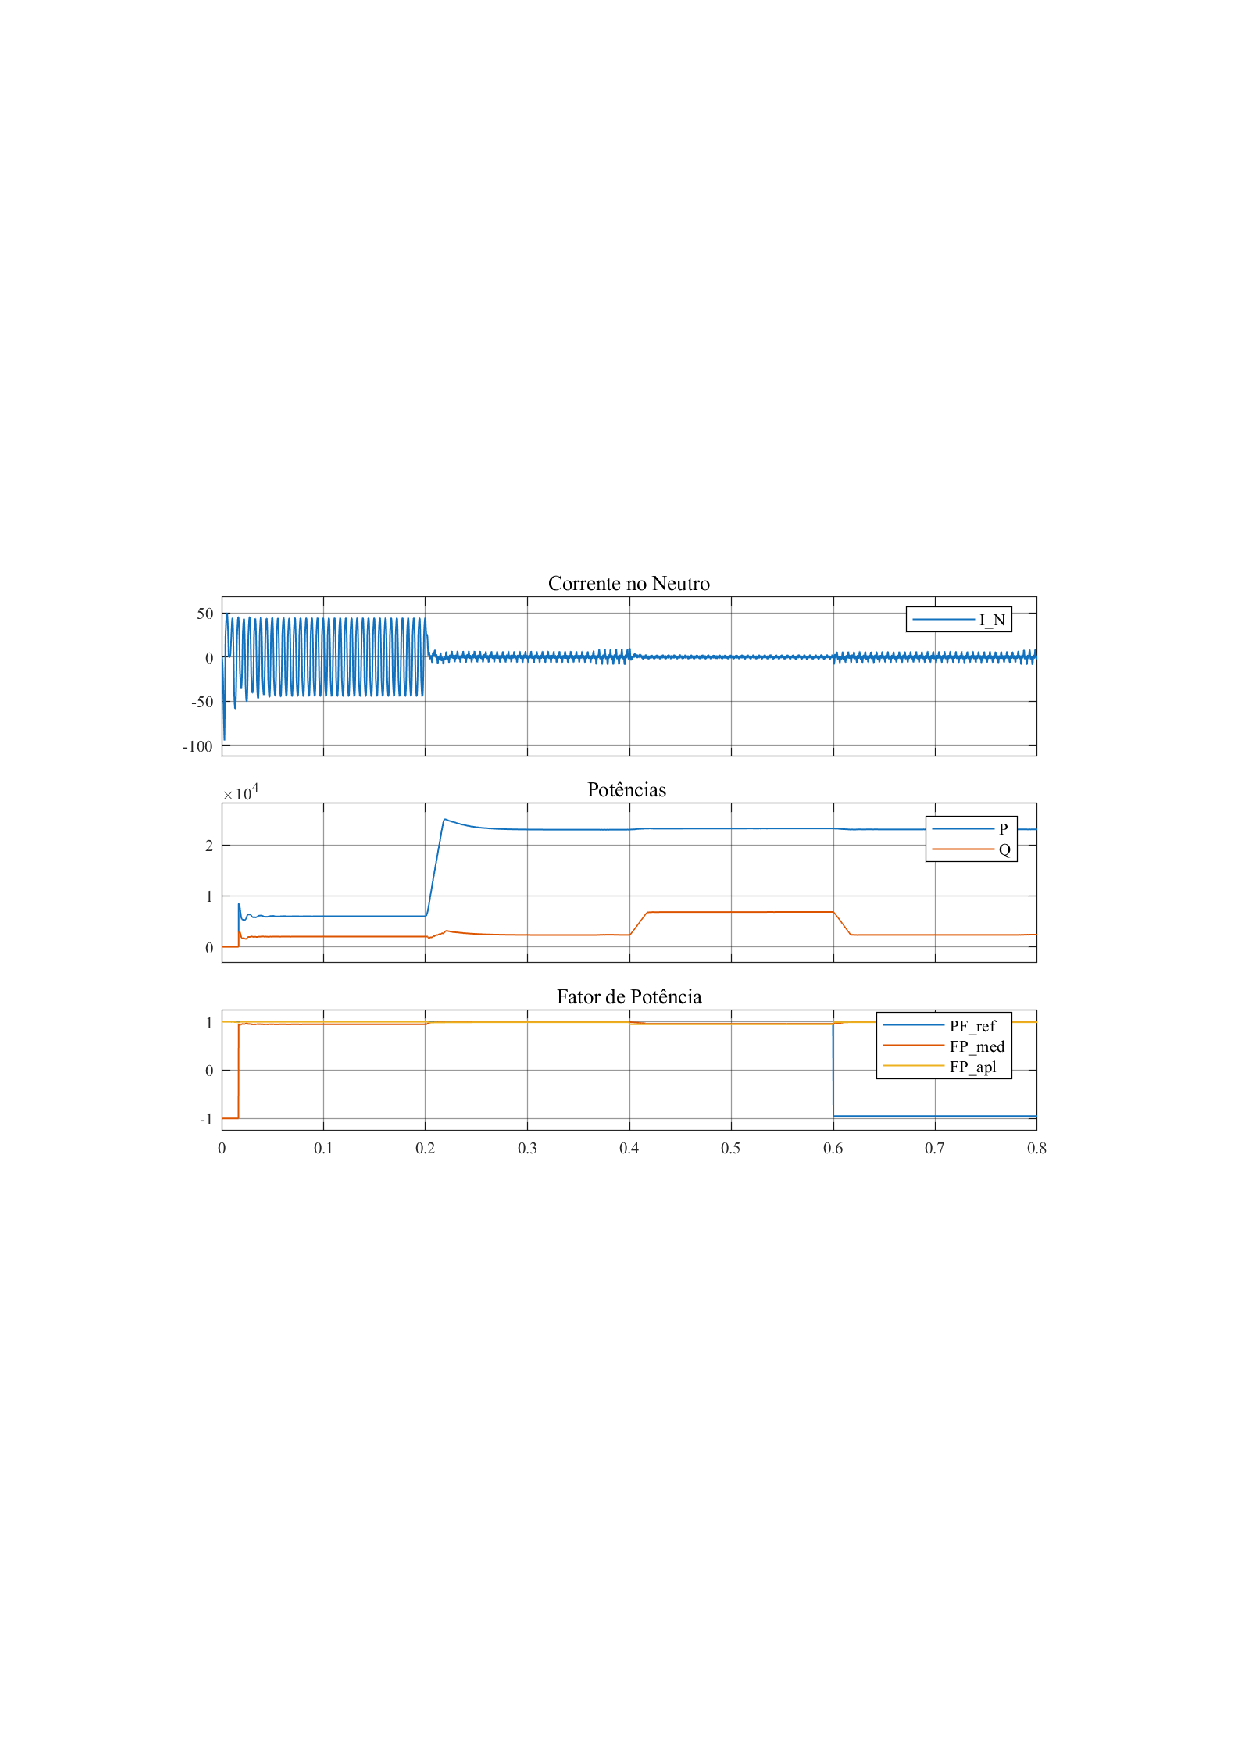
\includegraphics[width=\columnwidth, trim=87 272 87 272, clip]{Potencia2.pdf}
    \caption{Resultados da simulação para corrente no neutro, potências e FP com limitador ativado.}
    \label{fig:potencia}
\end{figure}

\begin{figure}[!t]
    \centering
    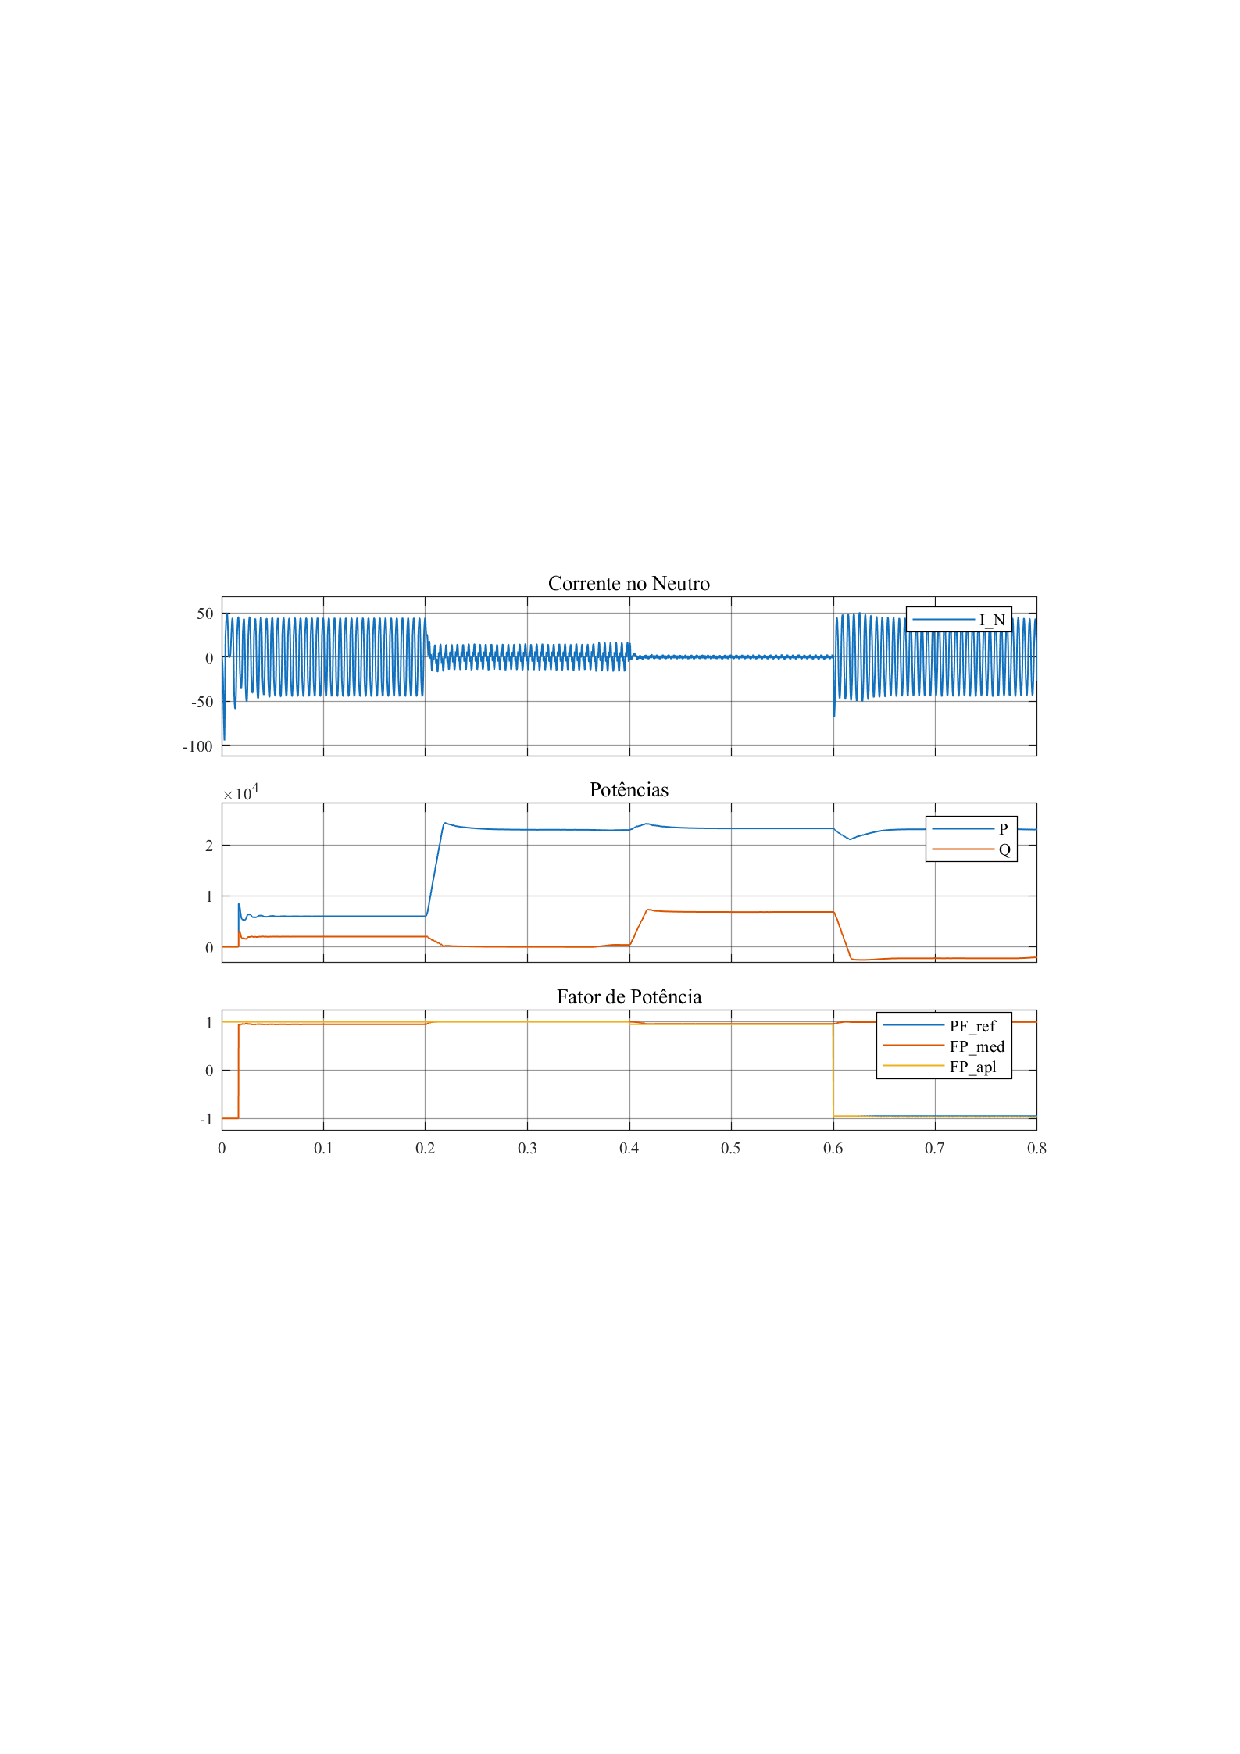
\includegraphics[width=\columnwidth, trim=87 272 87 272, clip]{Potencia2_semlim.pdf}
    \caption{Resultados da simulação para corrente no neutro, potências e FP sem limitador ativado.}
    \label{fig:potencia2}
\end{figure}

\begin{table}[!t]\centering\footnotesize\setlength{\tabcolsep}{3pt}
\caption{Valores de regime nos degraus de FP (carga nominal)}\label{tab:res}
\begin{tabular}{@{}ccccccc@{}}\toprule
\multirow{2}{*}{Intervalo} & \multirow{2}{*}{$\FP^*$} & \multirow{2}{*}{Lim.} & $\varphi$ apl./med. & $Q$ & FP & THD\\
 & & & [\si{\degree}] & [kvar] & medido & [\%]\\\midrule
\multirow{2}{*}{\SIrange{0,3}{0,4}{s}} & \multirow{2}{*}{1} & sim & 7,7/5,8 & 2,3 & 0,995 ind. & 3,1\\
 & & não & 0,0/0,5 & 0,2 & 1,000 & 7,8\\\midrule
\multirow{2}{*}{\SIrange{0,4}{0,6}{s}} & \multirow{2}{*}{0,95 ind.} & sim & 18,2/16,4 & 6,8 & 0,959 ind. & 0,3\\
 & & não & 18,2/16,4 & 6,8 & 0,959 ind. & 0,3\\\midrule
\multirow{2}{*}{\SIrange{0,6}{0,8}{s}} & \multirow{2}{*}{0,95 cap.} & sim & 7,7/5,8 & 2,3 & 0,995 ind. & 2,7\\
 & & não & $-14{,}5$/$-5{,}5$ & $-2{,}2$ & 0,995 cap. & 20,1\\\bottomrule
\end{tabular}\end{table}

\subsection{Operação com tensões distorcidas}

Para avaliar a operação com rede distorcida, foi adicionada à fonte, a partir de $t=\SI{0,3}{s}$, uma quinta harmônica de sequência negativa com \SI{5}{\percent} e
uma sétima harmônica de sequência positiva com \SI{3}{\percent} da fundamental, mantendo os intervalos de fator de potência como descritos para o caso anterior. Foram
simulados dois casos, um com as duas harmônicas na fase \ang{0} e outro com as duas harmônicas na fase \ang{180}. Em ambos os casos, os ângulos medidos e
as potências ativa e reativa permaneceram iguais às apresentadas na Tabela~\ref{tab:res}. Essa manutenção de resultados comprova o funcionamento
do rastreamento de ângulo do PLL.

No intervalo de $\FP^*=0{,}95$ indutivo, sem a atuação do limitador, o THD passou de \SI{0,3}{\percent} para \SI{1,3}{\percent} para as harmônicas em \ang{0} e para \SI{1,2}{\percent} para as harmônicas
em \ang{180}. Nos intervalos próximos à borda da janela de fator de potência estabelecida, notou-se que, para as harmônicas em \ang{0}, o THD caiu de \SI{3,1}{\percent} para \SI{1,5}{\percent} para $\FP^*=1$
e, na faixa capacitiva, foi de \SI{2,7}{\percent} para \SI{1,3}{\percent}; já com \ang{180}, os valores subiram para \SI{5,9}{\percent} e \SI{5,5}{\percent}, respectivamente. Isso ocorre porque as harmônicas
alteram a forma da tensão próxima à passagem por zero e, conforme a fase, encurtam ou alongam o trecho de sinais opostos na borda da janela. Sem a utilização do limitador,
para \ang{0}, o THD foi de \SI{6,2}{\percent} com $\FP^*=1$ e de \SI{19,5}{\percent} no pedido de fator de potência capacitivo. Dessa forma, percebeu-se que a vantagem do limitador
é mantida com a rede distorcida, mas, para o caso de distorções harmônicas na rede, a janela $\Delta$ escolhida para a rede senoidal não garante THD abaixo de
\SI{5}{\percent}.


\section{Discussão}
\label{sec:discussao}
Os resultados confirmam que a restrição de sinal de \eqref{eq:modelo_vienna4} define a faixa de FP do retificador a quatro fios. 
Como cada braço só aplica tensão com o mesmo sinal da corrente, a componente fundamental da tensão do conversor fica em fase com a corrente, e o conversor se comporta, para a rede, como uma resistência equivalente em série com o indutor de entrada. 
A rede passa então a fornecer o reativo do próprio indutor, $Q_L=\tfrac{3}{2}\omega_0LA^2$. Com $A\approx\SI{85}{A}$, tem-se $Q_L\approx\SI{6,1}{kvar}$ para $P\approx\SI{23}{kW}$, o que corresponde a $\psi_0=\arctan(Q_L/P)\approx\ang{15}$, valor coerente com \eqref{eq:phi} e com a janela de \ang{7} a \ang{23} empregada na simulação.

O retificador de Vienna a três fios opera com FP não unitário, indutivo ou capacitivo, com defasagem de até cerca de $\pm\ang{30}$~\cite{kolar2013essence}. 
Isso é possível porque, a três fios, somar uma mesma tensão de sequência zero às três referências não altera as correntes de fase. 
A quatro fios, a ligação entre o neutro e o ponto médio faz qualquer tensão de sequência zero circular como corrente pelo neutro, e essa liberdade deixa de existir: na região de sinais opostos, então, a tensão se torna nula, e o erro de tensão distorce a corrente. O FP capacitivo continua possível, porém essa operação ocorrerá com THD elevado, além de uma corrente de neutro elevada e reativo inferior ao pedido.

O limitador proposto segue a prática da literatura de não perseguir referências que a topologia não consegue sintetizar, como visto em \cite{liao2026nonunity} onde a referência de corrente é ajustada para evitar a região não sintetizável. A quatro fios, essa é uma das alternativas disponíveis para evitar a distorção. Dessa forma, a diferença entre $\FP^*$ e o FP medido após \SI{0,6}{s} apresentada na Fig.~\ref{fig:potencia} não indica falha do controle, mas a saturação de um pedido fora da região de operação.

Como $\sin\psi_0=\omega_0LA/V_{\sub{pk}}$, a posição da janela depende da reatância de entrada em pu. Com $L=\SI{1,5}{mH}$ (\SI{0,25}{pu} na base nominal do conversor), a janela fica deslocada para o lado indutivo. A capacitância não altera a janela, ela apenas define a ondulação do ponto médio, que é compensada pela ação antecipativa com $V_{C1}$ e $V_{C2}$ medidas e filtrada antes do PI de equilíbrio. A corrente de neutro também não se anula com o limitador, pois ainda há a ondulação de chaveamento, comum às três fases por usarem a mesma portadora, e pequenas harmônicas de terceira ordem que se somam no neutro.



\section{Conclusões}
\label{sec:conclusoes}

Este trabalho revisou as topologias CA--CC para carregadores
de VEs e estudou o retificador Vienna a quatro fios com FP
variável. O controle proposto, com PR por fase no referencial
estacionário e referência $A\cos(\theta-\varphi)$, permite variar o FP sem
perturbar a malha de tensão. Como a ligação do neutro elimina o grau de liberdade de modo comum, a faixa de FP sem distorção fica restrita a uma janela indutiva centrada
em $\psi_0 = \arcsin(\omega_0 L A/V_{\sub{pk}})$, que se desloca com a carga, e
pedidos fora dela, principalmente capacitivos, geram distorção
e corrente de neutro elevadas. O limitador proposto mantém a
operação dentro da janela, com THD de até \SI{3,1}{\percent}, e a diferença entre o FP pedido e o obtido indica quando o pedido
excede a capacidade da topologia analisada.



% ---------- Referências ----------
\printbibliography

% ---------- Anexos (opcional) ----------
%\appendices
%\section{Título do anexo}
Conteúdo opcional. Para usar, descomente \verb|\appendices| e o \verb|\input| no Main.tex.


\end{document}
